\chapter{Visão Estereoscópica - \textit{Stereo Imaging}}
\label{Revisão Bibliográfica}

% Dica:  Embasamento Teórico ou Fundamentação Teórica: revisão da literatura dos tópicos que sustentam a ciência e o conhecimento, relativos aos objetivos e aos métodos escolhidos para o desenvolvimento do trabalho.
% - Itens como Considerações Iniciais e Finais não são obrigatórios, mas completam muito bem qualquer capítulo.

%-----------------------------------------------------------------------------------------------------------------------------------------------------------------------------------------------
A visão estereoscópica possibilita uma boa identificação de um espaço tridimensional, visto que sua estrutura permite a triangulação de pontos chaves, assim determinando-se o seu correto posicionamento. Deste modo, compreende-se o porquê deste sistema visual ser amplamente difundido na evolução humana e animal. Em visão computacional, deseja-se emular os sistemas de visão mais eficientes para identificação de objetos e reconhecimento de ambientes. Computacionalmente, este processo pode ser realizado em quatro etapas: retificação,  Nas próximas seções encontram-se apresentadas o modelamento matemático, a triangulação, a calibração, a retificação e a projeção tridimensional para este tipo de sistema. 


%-----------------------------------------------------------------------------------------------------------------------------------------------------------------------------------------------
\section{Triangulação - \textit{Triangulation}}

Idealmente, a triangulação de um Ponto P de coordenadas globais (X,Y,Z) pode ser realizada caso tenha-se uma estrutura estéreo, cujas câmeras não apresentem distorção e estejam perfeitamente alinhadas. Deste modo, matematicamente, é possível abstrair os sensores das câmeras como dois planos coplanares entre si. Nessas condições, tem-se que os eixos ópticos das câmeras são paralelos. O eixo óptico, também conhecido como raio principal, é a reta que intercepta o ponto de centro de projeção ${O}$ e o ponto principal da lente ${c}$. Assumindo que as câmeras sejam exatamente iguais e alinhadas, tem-se que os pontos focais da câmera esquerda e da câmera direita são iguais ${f_l = f_r}$ e os pontos principais ${c^{left}_x}$ e  ${c^{right}_x}$ apresentam as mesmas coordenadas \cite{Bradski2008}. A figura \ref{stereo_image_geometric_model} ilustra a representação do modelo idealizado de um sistema estéreo.


\begin{figure}[H]
 	\centering
 	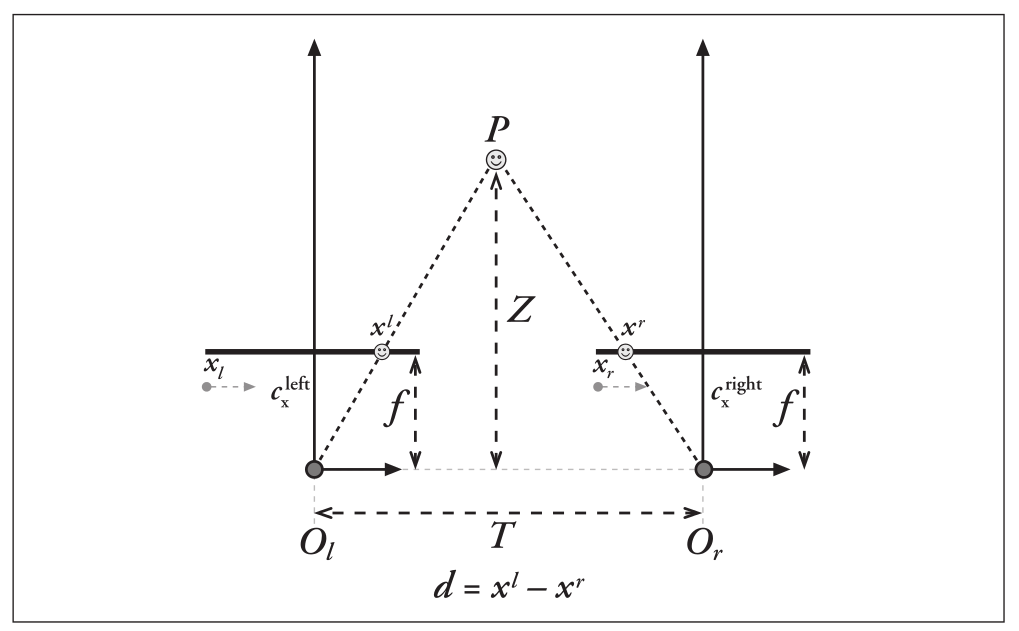
\includegraphics[scale=0.35]{./Resources/stereo_image_geometric_model.png}
 	\caption{Modelo Idealizado de um sistema de Visão Estéreo(Bradski,2008)}
 	\label{stereo_image_geometric_model}
\end{figure}


%-----------------------------------------------------------------------------------------------------------------------------------------------------------------------------------------------
\section{Geometria epipolar - \textit{Epipolar Geometry}}


%-----------------------------------------------------------------------------------------------------------------------------------------------------------------------------------------------
%\section{Calibração \textit{Stereo Calibration}}
%\subsection{Parâmetros intrínsecos}

%\subsection{Parâmetros extrínsecos}


%----------------------------------------------------------------------------------------------------------------------------------------------------------------------------------------------
%\section{Retificação de Imagens  - \textit{Stereo Rectification}}


%-----------------------------------------------------------------------------------------------------------------------------------------------------------------------------------------------
%\section{Correspondência Estéreo - \textit{Stereo Correspondence}}
%\subsection{BM}
%\subsection{SGBM}
%\subsection{BMGPU}

%-----------------------------------------------------------------------------------------------------------------------------------------------------------------------------------------------
\section{Mapa de disparidades - \textit{Disparity Map}}


%-----------------------------------------------------------------------------------------------------------------------------------------------------------------------------------------------
%\section{Projeção Tridimensional - \textit{3D Reprojection}}


%-----------------------------------------------------------------------------------------------------------------------------------------------------------------------------------------------
%\section{Reconhecimento de Objeto - \textit{Object Recognition}}
%\subsection{Segmentação - \textit{Image Segmentation}}

%\subsection{Identificação - \textit{Object Identification}}

%-----------------------------------------------------------------------------------------------------------------------------------------------------------------------------------------------
\section{Aplicações em Robótica}

Nesta seção, serão apresentados alguns dos trabalhos que têm como principais sensores ou utilizam câmeras estereoscópicas para a navegação autônoma em ambientes terrestre, aérea e subaquática.

Nos dias de hoje, as empresas automobilísticas vem participando de uma verdadeira corrida tecnológica para o desenvolvimento de automóveis totalmente autônomos e economicamente viáveis. As universidades não ficaram para trás e também apresentam pesquisas envolvendo desenvolvimento de algoritmos de controle e sensores, tornando essa corrida ainda mais acirrada. Os resultados apresentados são realmente promissores, o que concretizam cada vez mais essa realidade tida até então como distante. Na figura \ref{caminhao_autonomo} abaixo, é possível observar o projeto de caminhão autônomo desenvolvido pelo Laboratório de Robótica Móvel - LRM - ICMC/USP. O caminhão conta com diversos sensores, dentre eles câmeras estereoscópicas, que identificam outros automóveis, pessoas e faixas de sinalização \cite{ShinzatoP}. 

\begin{figure}[H]
 	\centering
 	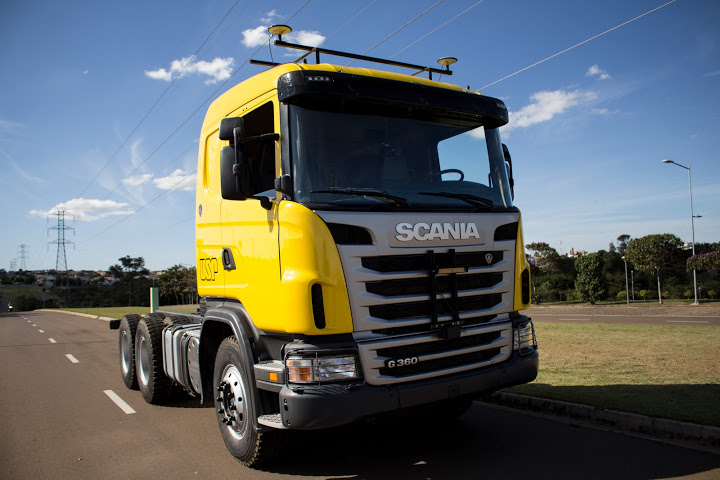
\includegraphics[scale=0.35]{./Resources/caminhao_autonomo.jpg}
 	\caption{Caminhão Autônomo desenvolvido pelo Laboratório de Robótica Móvel - LRM - ICMC/USP em parceria com a Scania}
 	\label{caminhao_autonomo}
\end{figure}

No caso de navegação autônoma para ambiente aéreo, o projeto utilizando \textit{Micro Air Vehicle} (MAVS) desenvolvido pelo \textit{Massachusetts Institute of Technology} (MIT) permite que estas pequenas aeronaves consigam navegar autonomamente e desviar de obstáculos voando a um velocidade de 30 mph (48 $km/h$). A figura \ref{mit_drones} abaixo apresenta o trabalho desenvolvido, o qual é um comparativo de desempenho de uma implementação em hardware utilizando \textit{Field-programmable gate array} (FPGA) e um processador ARM para processamento embarcado do método \textit{Semi-Global Block Matching} (SGBM) \cite{BarryMIT}.

\begin{figure}[H]
 	\centering
 	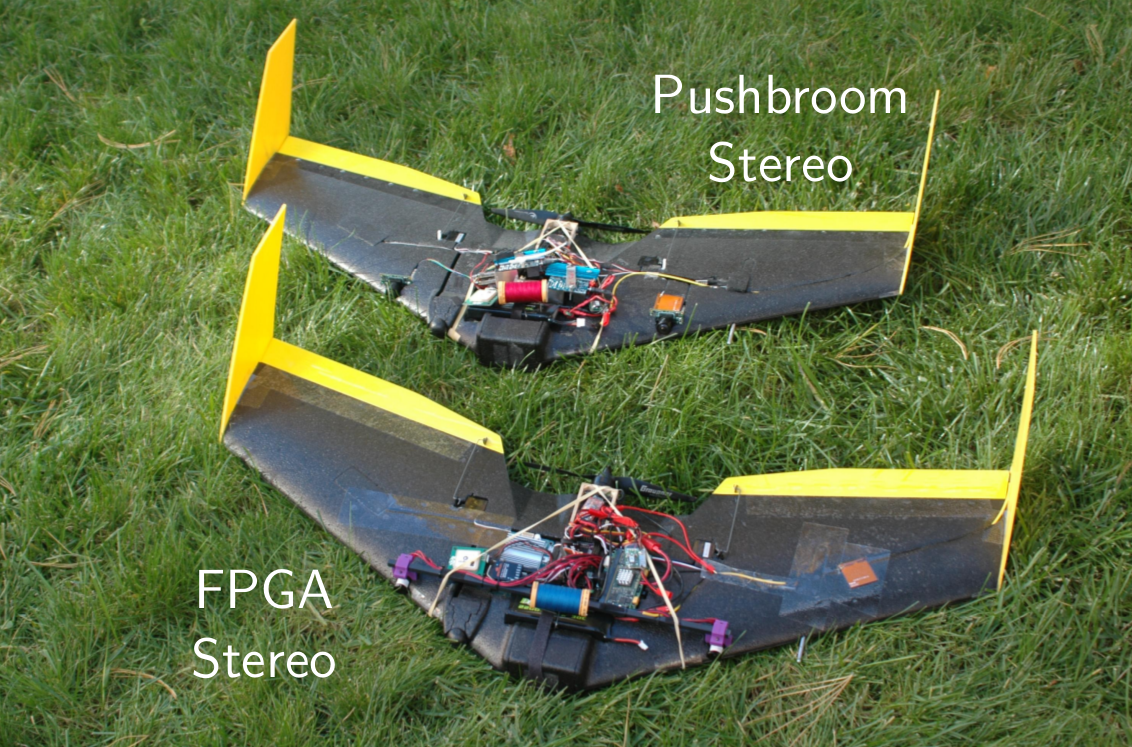
\includegraphics[scale=0.30]{./Resources/mit_drones.png}
 	\caption{Plataformas experimentais de aeronaves com o Sistema Estéreo - FPGA (frente) e o Sistema Estéreo - Pushbroom (trás). Câmaras são montados na parte dianteira das asas na mesma linha de base (34 cm) em ambas células.}
 	\label{mit_drones}
\end{figure}

No caso de navegação autônoma para ambiente subaquático, um exemplo de \textit{autonomous underwater vehicle} (AUV) é o projeto desenvolvido pela Universidade espanhola de Girona (veja figura \ref{G500}). O trabalho propõe a utilização do método de Mapeamento e Localização Simultânea (SLAM),juntamente com câmeras estereoscópicas, para o reconhecimento do ambiente, aprimorando assim o erro de rastreamento dos objetos \cite{Nagappa2013}.

\begin{figure}[H]
 	\centering
 	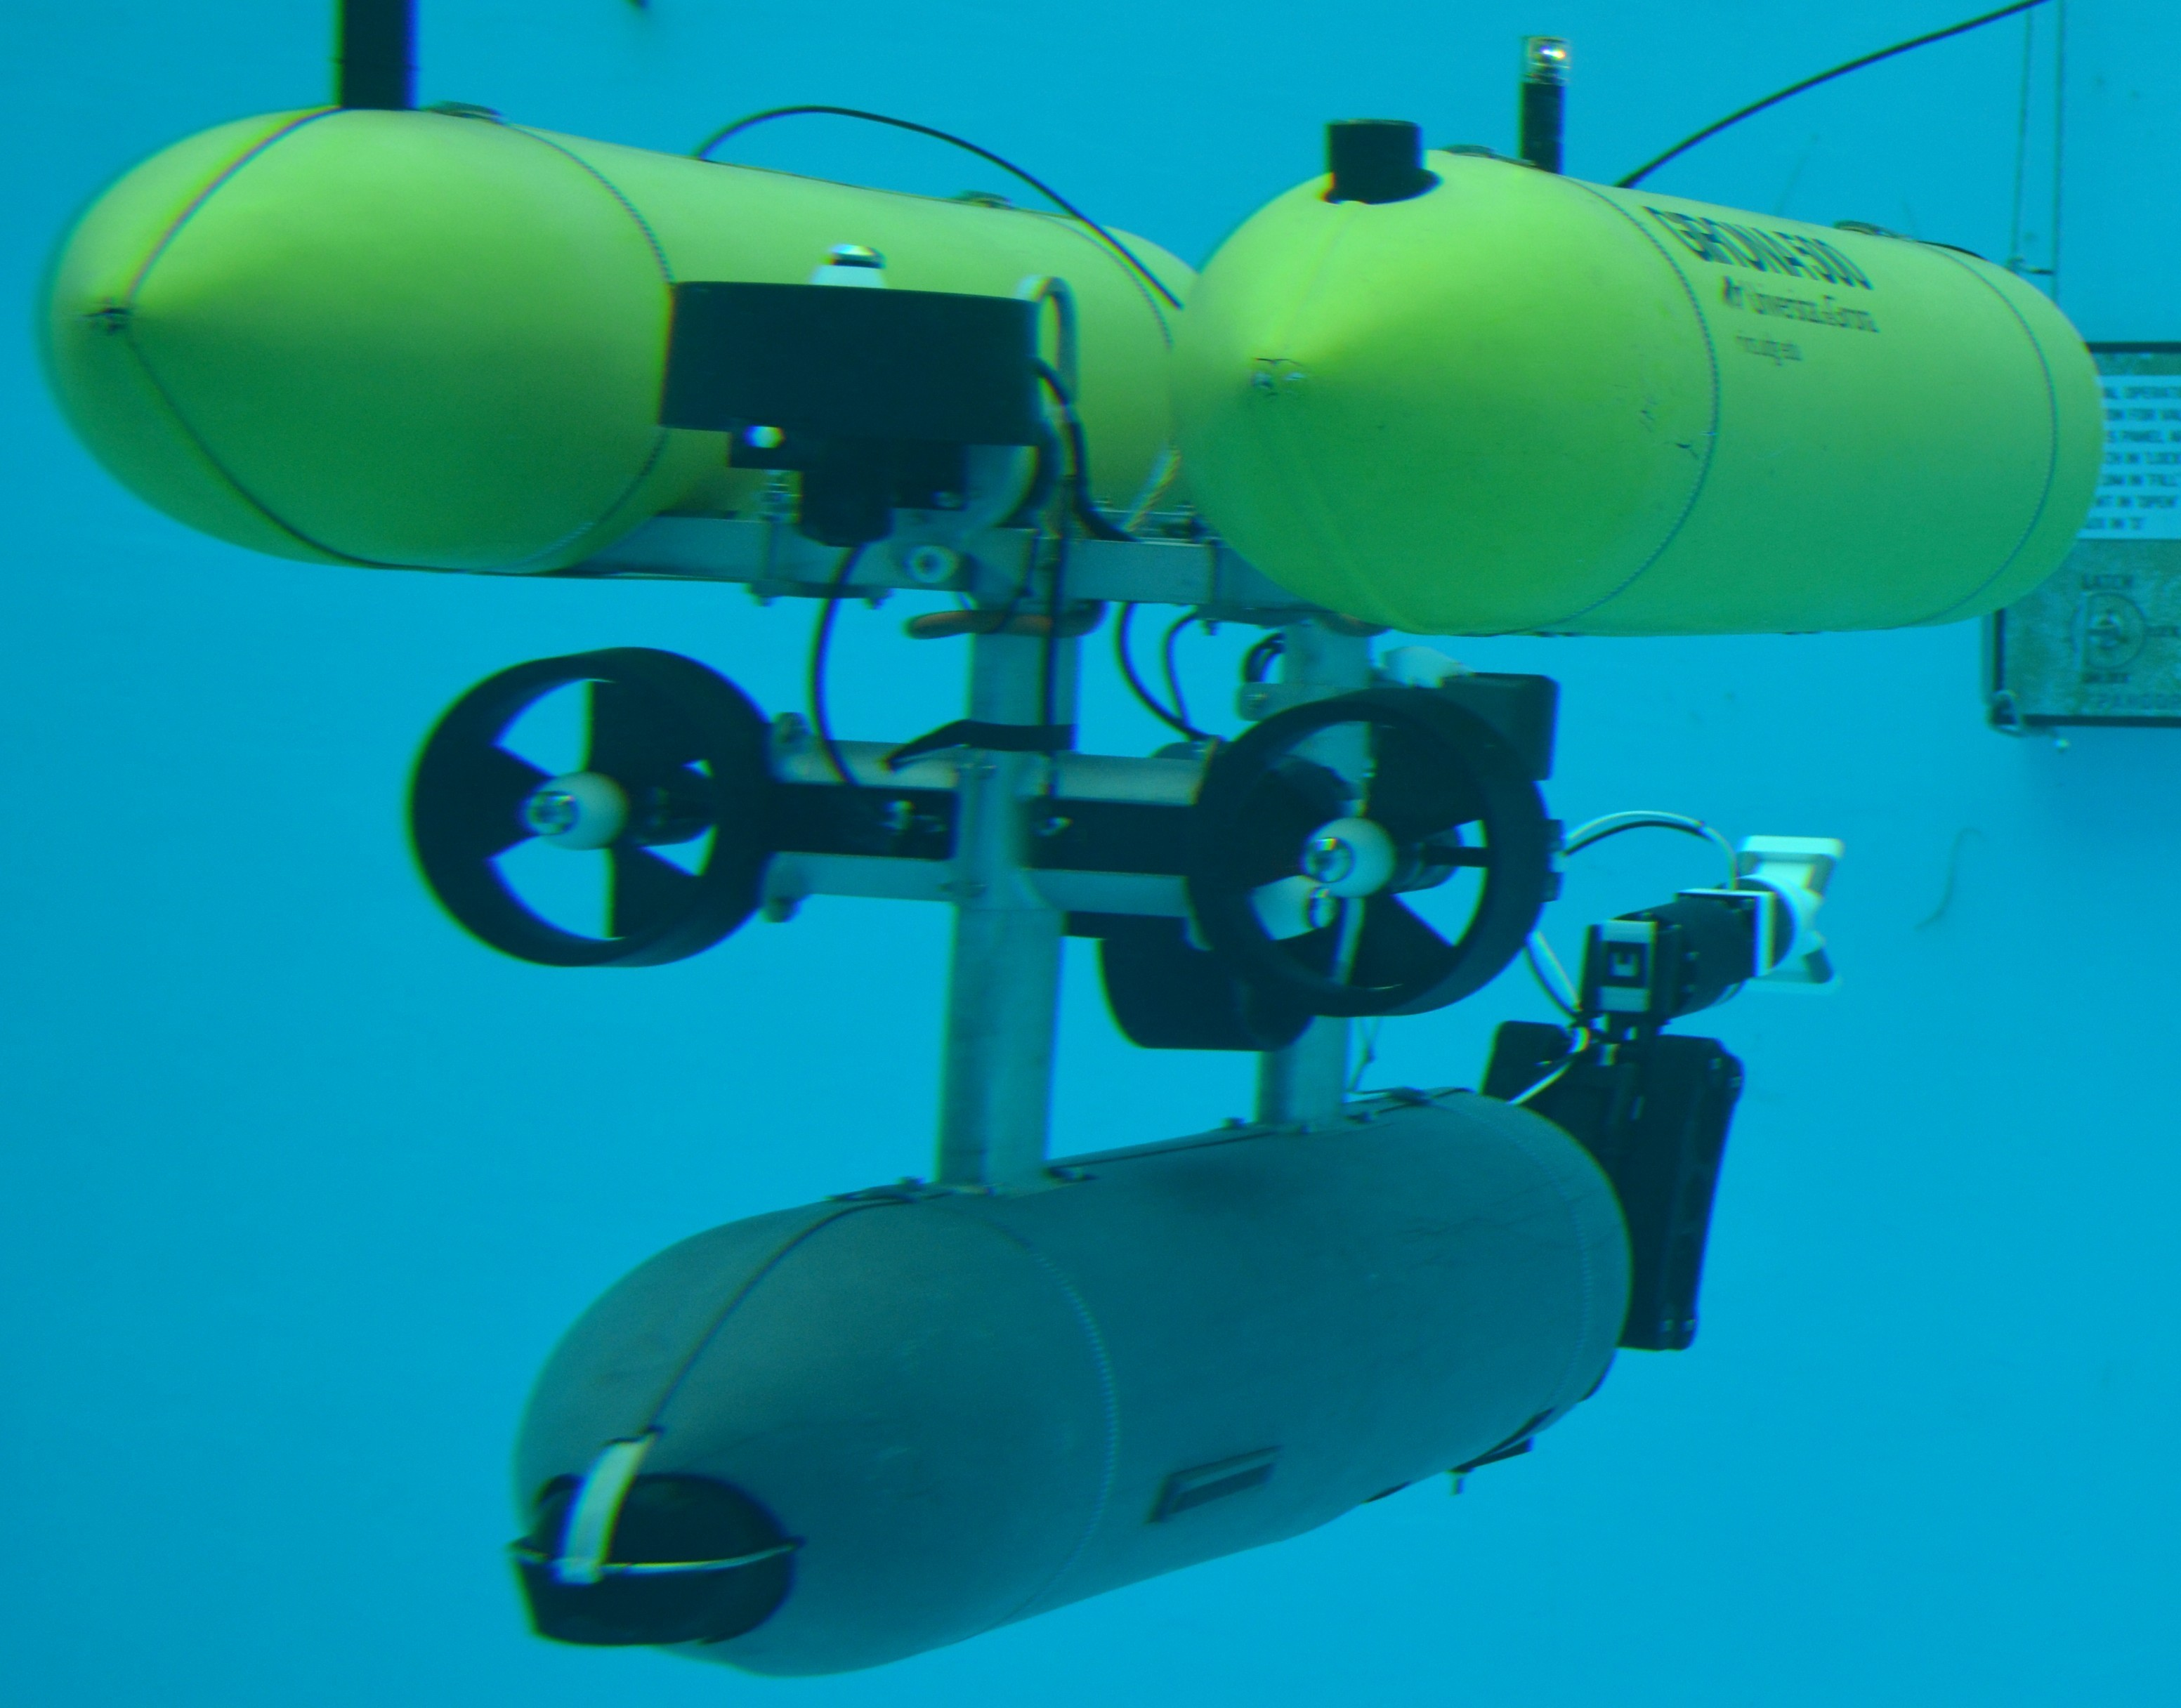
\includegraphics[scale=0.1]{./Resources/G500.jpg}
 	\caption{Veículo Submarino Autônomo - Girona 500}
 	\label{G500}
\end{figure}


%-----------------------------------------------------------------------------------------------------------------------------------------------------------------------------------------------